\chapter{I Moti Relativi}

\section{Introduzione}

Agli spostamenti, alle velocit\`a, con le quali abbiamo
or ora fatto conoscenza, e, con prudenza, alle accelerazioni calza spesso a pennello
l'epiteto ``relativo''.
Stando seduti sul sedile di un treno che si muove per partire
dalla stazione in molti hanno sperimentato
la percezione che un altro treno, vicino di binario al nostro,
si stesse muovendo verso il fondo delle rotaie, in procinto
di scendere i gradini verso Piazza Duca d'Aosta\footnote
{
Per chi parte dalla Stazione Centrale di Milano.
}.
Un tale dubbio non potrebbe mai sorgere
nella mente
di un passeggero di quel treno che invece ci osserva tranquillamente partire.  
Come pure, rimanendo in ambito ferroviario, il passeggero che cammina placido
verso la testa del treno possiede, rispetto ad un passeggero a terra, che aspetta 
sul marciapiede,
la propria velocit\`a sommata a quella del treno.


\begin{figure}[ht]
	\begin{center}
      		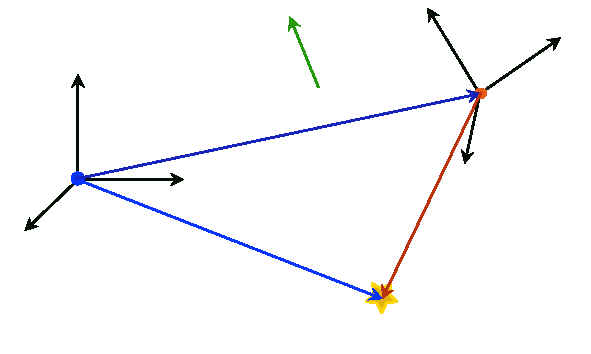
\includegraphics{part1/relativi/FIG/f19.pdf}
	\end{center}
\begin{picture}(0,0)(-55,-50)
\scriptsize{
	\put(0,66){$\scriptscriptstyle{\rm {Terra}}$}
	\put(162,-10){$\scriptscriptstyle{\rm {Sole}}$}
	\put(220,98){\rotatebox{35}{$\scriptscriptstyle{\rm {Marte}}$}}
	\put(110,72){$\bm{d}$}
	\put(80,26){$\bm{s}_{\scriptscriptstyle{T}}$}
	\put(188,36){$\bm{s}_{\scriptscriptstyle{M}}$}
	\put(135,125){$\bm{\Omega}$}
}
\end{picture}
\vskip -6mm
	\caption{\em Osservazione del Sole da due pianeti diversi.}
     \label{fig:f19}
\end{figure}

\noindent Insomma, gli spostamenti di un oggetto,
come anche le sue velocit\`a e le sue accelerazioni, appaiono
diversi ad osservatori tra loro in movimento. Anzi tutte le grandezze cinematiche sono
legate (relative) all'osservatore che le misura. La domanda che ci si pu\`o porre, 
la quale costituisce il
{\em problema dei moti relativi}\index{problema dei moti relativi},
\`e la seguente: risulta possibile a due diversi osservatori scambiare i dati
provenienti dalle loro indagini cinematiche e confrontare le rispettive osservazioni
eseguite sopra oggetti comuni? La risposta \`e s\`i, stando a certi patti e a certe condizioni.

\section{Posizione del Problema}
Premettendo che una trattazione del {\em teorema di Coriolis}, rigorosa e completa, si trova
magistralmente esposta nel gi\`a citato \cite{finzi}, pag. 219, riportiamo qui un esempio che 
riteniamo un inquadramento piuttosto generale del {\em problema dei moti relativi}.
Un terrestre e un marziano,
di professione astronomi, sono appassionati di osservazioni solari:
entrambi misurano con facilit\`a posizione, velocit\`a e accelerazione della nostra 
stella. Nessuna delle quantit\`a misurate dal terrestre \`e in accordo con la
corrispondente del marziano\footnote{Un caro amico, leggendo le bozze di questo lavoro,
mi ha fatto notare come, pur lasciando da parte il sapore vagamente tolemaico
delle misure di velocit\`a e accelerazione del Sole da parte dei due astronomi,
 non sia comunque possibile il confronto tra  osservazioni
eseguite da due distinti punti dell'universo separati da immense distanze, in quanto
la luce del Sole impiega tempi rilevanti e diversi per giungere sulla Terra e su Marte.
Rispondiamo a questa giusta critica affermando che,
 fuori dalla sfera dei meccanismi, dove gli esempi di moti relativi abbondano,
purtroppo non ci vengono in mente
altre situazioni da proporre, sia pure di fantasia.
Per questo ci teniamo gli astronomi tolemaici,
 supponendo in tutto questo che la velocit\`a della luce sia infinita.}.
 Il terrestre, forse per protagonismo, decide di misurare
alcune quantit\`a cinematiche di Marte, {\em in primis} la sua posizione $\bm d$ e le 
corrispondenti
derivate ma,
incuriosito dalla rotazione del suo corrispondente (dispongono di cannocchiali potentissimi), decide di misurare anche
$\bm \Omega$, la velocit\`a angolare di Marte rispetto alla Terra.
Mediante lo schema fornito dalla figura
\ref{fig:f19}, impostano la seguente relazione
\begin{equation}
	\bm{s}_{\scriptscriptstyle{T}}=
	\bm{d}+
	\bm{s}_{\scriptscriptstyle{M}}\,,
\label{e128}
\end{equation}
\noindent che infonde ai due astronomi (sono ovviamente in contatto tra loro)
un pizzico di ottimismo circa la loro relazione, perch\'e la trovano soddisfatta.
Il terrestre ha a disposizione anche la velocit\`a del punto di Marte dove lavora il suo
amico extraterrestre,
$\dot{\bm d}$, e il marziano gli fornisce gentilmente la sua misura della
velocit\`a del Sole,
$\dot{\bm{s}}_{\scriptscriptstyle{M}}$.
Ma scrivendo la seguente
\begin{equation}
\xcancel{\dot{\bm{s}}_{\scriptscriptstyle{T}}=
	\dot{\bm{d}}+
\dot{\bm{s}}_{\scriptscriptstyle{M}}}\,,
\label{e129}
\end{equation}
\noindent in apparente accordo con la \ref{e128}, e sostituendo dati in loro
possesso, incontrano una cocente delusione.
Con lo scopo di rendere pi\`u chiare le interazioni future tra i due osservatori
conviene attribuire loro epiteti che ricordino le loro ``prerogative''. A ben 
considerare, essi sono completamente intercambiabili: Marte e Terra sono
due pianeti a pieno titolo e nessuno dei due osservatori
possiede caratteristiche tali da
implicare alcuna sorta di privilegio. Chiameremo tuttavia
{\em osservatore assoluto}\index{osservatore!assoluto} colui che
misura, oltre alle grandezze cinematiche del Sole,
anche le grandezze cinematiche dell'altro osservatore, che sono il
vettore $\bm d$, il vettore $\bm \Omega$ e le loro derivate; per noi costui \`e,
ad arbitrio, l'osservatore terrestre.
Chiameremo invece
il marziano {\em osservatore relativo}\index{osservatore!relativo}.
Risulta chiaro da quanto ora esposto che i due ruoli sono invertibili:
basterebbe all'osservatore marziano essere in possesso di posizione,
velocit\`a e accelerazione, grandezze angolari comprese, della
Terra per potere diventare 
l'osservatore assoluto.
\noindent Il terrestre pensa e ripensa alla \ref{e129} e, cercando di capire dove
si nasconde l'errore, per stanarlo conduce il seguente esperimento mentale: immagina una mosca
aliena ferma sulla lente del cannocchiale marziano e, con lo scopo
di conoscerne la velocit\`a, prova ad applicare a
essa l'errata 
formula \ref{e129}. La {\em velocit\`a relativa}\index{velocit\`a!relativa},
cio\`e la velocit\`a della mosca misurata dal marziano, quella che nella 
\ref{e129} \`e indicata con 
$\dot{\bm{s}}_{\scriptscriptstyle{M}}$,
 \`e in questo caso sicuramente nulla.
Per tale ragione, l'osservatore assoluto (il terrestre) si dovrebbe accontentare di ottenere
per la velocit\`a della mosca, come per le velocit\`a di tutti gli oggetti fermi
 su Marte, un valore uguale a
$\dot{\bm{d}}$. Ebbene questo sarebbe possibile solo se tali oggetti (i
punti considerati di tali oggetti) si trovassero giusto
nel centro della terna del sistema di riferimento marziano, oppure se tutto il pianeta,
e di conseguenza il sistema di riferimento a esso collegato, traslasse.
\noindent Addebitando alla rotazione del sistema relativo la causa delle differenti velocit\`a assolute
degli oggetti fermi su Marte cominciano a intravedere uno
spiraglio di luce verso la soluzione dell'enigma. La formula
\ref{e129} non funziona perch\'e il sistema di riferimento relativo ruota rispetto
al sistema di riferimento assoluto con velocit\`a angolare $\bm \Omega$. Per  stimare
 l'errore
che l'osservatore relativo commette nell'effettuare ``le proprie derivate'' l'osservatore
assoluto chiede al marziano di comunicargli
la derivata di un vettore $\bm a$
di modulo costante e fisso con il sistema assoluto.
Il marziano vede tale vettore
ruotare con velocit\`a angolare $-\bm \Omega$ e ne
determina una variazione temporale (derivata rispetto al tempo)
 pari a $\dot{\bm a}= - {\bm \Omega}\times {\bm a}$.
\noindent Il calcolo di questo termine \`e gi\`a stato svolto in precedenza, nel capitolo
in cui si descrivono gli spostamenti infinitesimali, e in
quel contesto \`e limitato al caso
piano, equazioni \ref{e14}, \ref{e15}, \ref{e16}.
A questo punto l'osservatore assoluto conosce il termine correttivo da introdurre 
nella \ref{e129} e la riscrive correttamente\footnote
{
Per coloro i quali volessero approfondire il calcolo delle
derivate di un vettore rotante o, ci\`o che \`e lo stesso, la relazione
tra la rotazione del sistema di riferimento e la variazione (apparente)
di un vettore, rimandiamo a \cite{finzi}, pag. 163.
}
\begin{equation}
\dot{\bm{s}}_{\scriptscriptstyle{T}}=
	\dot{\bm{d}}+
\dot{\bm{s}}_{\scriptscriptstyle{M}}+
 {\bm \Omega}\times 
	\bm{s}_{\scriptscriptstyle{M}}\,.
\label{e130}
\end{equation}

\noindent Le velocit\`a dei punti che sono fermi su Marte, come la mosca sulla lente del
cannocchiale, assumono il nome speciale di {\em velocit\`a di trascinamento}\index{velocit\`a!di trascinamento}
\begin{equation}
{\bm v}_{\scriptscriptstyle{{\rm tr}}}=
	\dot{\bm{d}}+
 {\bm \Omega}\times 
	\bm{s}_{\scriptscriptstyle{M}}\,,
\label{e131}
\end{equation}
ovviamente variabile da punto a punto del sistema relativo.
\noindent La rimanente componente si chiama {\em velocit\`a relativa}\index{velocit\`a!relativa}
\begin{equation}
{\bm v}_{\scriptscriptstyle{{\rm rel}}}=
\dot{\bm{s}}_{\scriptscriptstyle{M}}\,,
\label{e132}
\end{equation}
\noindent che, sommata alla precedente, permette di ottenere
la {\em velocit\`a assoluta}\index{velocit\`a!assoluta}
del Sole 
\begin{equation}
{\bm v}_{\scriptscriptstyle{{\rm ass}}}=
{\bm v}_{\scriptscriptstyle{{\rm rel}}}+
{\bm v}_{\scriptscriptstyle{{\rm tr}}}\,.
\label{e133}
\end{equation}
\section{L'Accelerazione di Coriolis}

\noindent Giunti sin qui, sapendo che ogni derivata che provenga dal sistema relativo va depurata
aggiungendo il termine opportuno, i due astronomi provano a sostituire i loro
dati di accelerazione del Sole nella derivata della \ref{e130}
\begin{equation}
\ddot{\bm{s}}_{\scriptscriptstyle{T}}=
	\ddot{\bm{d}}+
\ddot{\bm{s}}_{\scriptscriptstyle{M}}+
 {\bm \Omega}\times 
\dot{\bm{s}}_{\scriptscriptstyle{M}}+
\dot{\bm \Omega}\times 
	\bm{s}_{\scriptscriptstyle{M}}+
 {\bm \Omega}\times 
\dot{\bm{s}}_{\scriptscriptstyle{M}}+
 {\bm \Omega}\times( 
 {\bm \Omega}\times 
	\bm{s}_{\scriptscriptstyle{M}})\,;
\label{e134}
\end{equation}
\noindent la quale sostituzione riempie di gioia i due astronomi perch\'e la
\ref{e134} viene soddisfatta: essi battezzano questa formula 
{\em teorema di Coriolis}\index{teorema!di Coriolis}. D'altra parte, una volta imparato a correggere le 
derivate provenienti dall'osservatore relativo, la \ref{e134} si ottiene
meccanicamente e senza impiego di gran ragionamenti derivando la \ref{e130}.
Anche in questo caso, come abbiamo fatto per le velocit\`a,
 conviene dare un nome speciale all'accelerazione 
dei punti fermi costantemente rispetto al sistema relativo (la mosca di 
poco fa ferma sulla lente del cannocchiale), e chiameremo 
{\em accelerazione di trascinamento}\index{accelerazione!di trascinamento} la seguente
\begin{equation}
{\bm a}_{\scriptscriptstyle{{\rm tr}}}=
	\ddot{\bm{d}}+
\dot{\bm \Omega}\times 
	\bm{s}_{\scriptscriptstyle{M}}+
 {\bm \Omega}\times( 
 {\bm \Omega}\times 
        \bm{s}_{\scriptscriptstyle{M}})\,.
\label{e135}
\end{equation}
\noindent Nella \ref{e135} compaiono solamente i termini della \ref{e130} che non contengono
grandezze cinematiche relative, n\'e velocit\`a n\'e accelerazioni (la mosca \`e ferma e rimane ferma).
L'{\em accelerazione relativa}\index{accelerazione!relativa} \`e naturalmente
\begin{equation}
{\bm a}_{\scriptscriptstyle{{\rm rel}}}=
\ddot{\bm{s}}_{\scriptscriptstyle{M}}\,,
\label{e136}
\end{equation}
\noindent ed \`e l'unica che l'osservatore relativo \`e in grado di misurare.
Della \ref{e130} restano due monomi, uguali, contenenti grandezze relative e grandezze
assolute  mescolate. L'espressione
\begin{equation}
{\bm a}_{\scriptscriptstyle{{\rm cor}}}=
2 {\bm \Omega}\times 
\dot{\bm{s}}_{\scriptscriptstyle{M}}=
2 {\bm \Omega}\times 
{\bm v}_{\scriptscriptstyle{{\rm rel}}}
\label{e137}
\end{equation}
\noindent si chiama {\em accelerazione di Coriolis}\index{accelerazione!di Coriolis}, in onore al matematico francese
{\em Gaspard-Gustave de Coriolis} che l'ha scoperta.
A questo punto, possiamo finalmente scrivere l'espressione
dell'{\em accelerazione assoluta}\index{accelerazione!assoluta}
nel modo seguente
\begin{equation}
{\bm a}_{\scriptscriptstyle{{\rm ass}}}=
{\bm a}_{\scriptscriptstyle{{\rm rel}}}+
{\bm a}_{\scriptscriptstyle{{\rm tr}}}+
{\bm a}_{\scriptscriptstyle{{\rm cor}}}\,.
\label{e138}
\end{equation}

\section{Riepilogo}

\noindent  Quando due osservatori,
in moto tra loro, indagano sulla cinematica di un terzo oggetto ne traggono
quantit\`a distinte. Per potere confrontare tali quantit\`a occorre che uno degli
osservatori (assoluto) misuri anche le quantit\`a cinematiche assolute
attribuibili al sistema relativo cio\`e
$\bm d$, $\bm \Omega$ e le loro derivate.
Alla velocit\`a di una formica (punto osservato), misurata dall'osservatore
relativo, l'osservatore assoluto dovr\`a aggiungere la componente di trascinamento
che \`e la velocit\`a assoluta del punto del sistema relativo dove la formica appoggia le 
zampe in quel momento.
Con le accelerazioni le cose vanno diversamente: non \`e sufficiente sommare la componente
del trascinamento all'accelerazione relativa per ottenere l'accelerazione assoluta. La
velocit\`a relativa provoca nei sistemi rotanti un'altra accelerazione,
detta di {\em Coriolis}, da aggiungere a quella relativa e di trascinamento, della quale
daremo nel seguente capitolo qualche ulteriore delucidazione.
\newpage
\thispagestyle{empty}
\null

\chapter{Esempi di Moti Relativi}

\section{Precisazioni sull'Accelerazione di Coriolis} 

\begin{figure}[h]
\centering
\begin{minipage}[b]{0.50\textwidth}
\centering
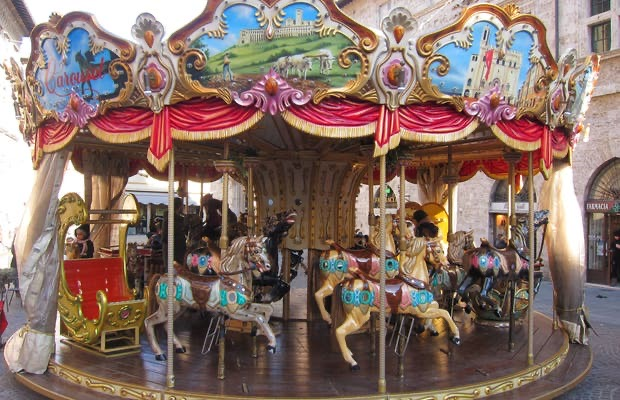
\includegraphics[width=0.9\textwidth]{part1/relativi/FIG/f110.jpg}
\caption{\em La giostra dei cavalli.}
 \label{fig:f110}
\end{minipage}\hfill
\begin{minipage}[b]{0.50\textwidth}
\centering
      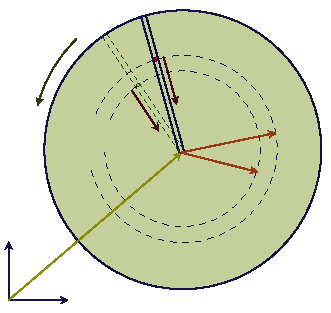
\includegraphics[width=0.9\textwidth]{part1/relativi/FIG/f111.pdf}
\begin{picture}(0,0)(130,0)
\scriptsize{
\put(24,131){${\rm d}\theta$}
\put(-19,116){$\omega$}
\put(-14,30){${\bm d}$}
\put(-29,32){$y$}
\put(-8,10){$x$}
\put(-3,86){${{\bm v}_{\scriptscriptstyle{{\rm rel}}}}(t+{\rm d}t)$}
\put(51,108){${{\bm v}_{\scriptscriptstyle{{\rm rel}}}}(t)$}
\put(60,66){$r-{\rm d}r$}
\put(70,85){$r$}
}
\end{picture}
        \caption{\em Versione schematica.}
     \label{fig:f111}
\end{minipage}
\end{figure}

\noindent La ``giostra dei cavalli'' sembra un laboratorio appositamente costruito per
fare esercizio coi moti relativi.
Essa ci riconduce innanzitutto ai nostri moti piani, dove l'intuito pu\`o meglio padroneggiare
la situazione.
Divertimento per bambini (e non) molto conosciuto, questa giostra si presenta come un grande
piatto rotante, normalmente pavimentato in legno, dove un paio di ranghi
di sedili, cavalli, carrozze e altro ospitano i turisti portandoli in rotazione. Credo che
i modelli pi\`u lussuosi muovano i cavalli anche verticalmente, ma questo non 
importa al nostro scopo, tant'\`e che ci\`o di cui misureremo le quantit\`a cinematiche,
cio\`e il nostro punto osservato, sar\`a una formica intenzionata a esplorare 
la giostra. L'osservatore assoluto potrebbe essere
il bigliettaio ed \`e rappresentato dal riferimento $(x,y)$, coincidente con la sua edicola.
\`E appena il caso di chiarire che il vettore
 ${\bm d}$ \`e costante perch\'e il centro della giostra
\`e fermo rispetto alla piazza, per questo motivo ${\bm d}$
non giocher\`a alcun ruolo nei ragionamenti che seguiranno.
Un turista seduto sulla giostra \`e nei panni dell'osservatore
relativo e, indagando il movimento della formica, riuscir\`a a misurare
la velocit\`a e l'accelerazione relative dell'insetto.
La velocit\`a e l'accelerazione del punto del pavimento dove si trova la formica
forniscono subito
le diverse componenti del trascinamento: tali quantit\`a cinematiche
appartengono ai punti del disco rotante.
Supponiamo ora che la formica si incammini lungo una fessura radiale
della pavimentazione, comune nelle giostre col {\em parquet}, come mostrato in figura \ref{fig:f111}.
Nell'istante di tempo considerato, sia ${{\bm v}_{\scriptscriptstyle{{\rm rel}}}}(t)$
la velocit\`a relativa della formica, cio\`e la velocit\`a con cui sta percorrendo l'interstizio
rettilineo. Si pu\`o osservare nella stessa figura che la circonferenza del
piatto della giostra dove si trover\`a la formica dopo un intervallo infinitesimale
di tempo ${\rm d}t$ avr\`a
un raggio minore. \`E naturale pertanto
pensare che, con riferimento ai due istanti considerati,
si avr\`a una differenza tra le due
velocit\`a di trascinamento cui sar\`a soggetta la formica.

\begin{figure}[hbt]
\centering
\begin{minipage}[b]{0.57\textwidth}
\centering
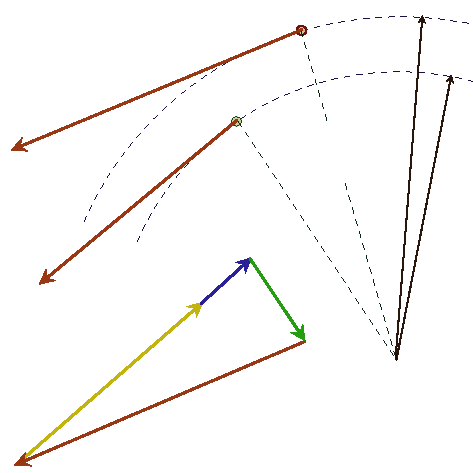
\includegraphics[width=0.8\textwidth]{part1/relativi/FIG/f112.pdf}
\begin{picture}(0,0)(130,0)
\scriptsize{
\put(59,108){${\rm d}\theta=\omega{\rm d}t$}
\put(-10,132){${{\bm v}_{\scriptscriptstyle{{\rm tr}}}}(t)$}
\put(-40,59){${{\bm v}_{\scriptscriptstyle{{\rm tr}}}}(t+{\rm d}t)$}
\put(101,147){$r$}
\put(118,100){$r-{\rm d}r$}
\put(-36,41){$-{{\bm v}_{\scriptscriptstyle{{\rm tr}}}}(t+{\rm d}t)$}
\put(10,12){${{\bm v}_{\scriptscriptstyle{{\rm tr}}}}(t)$}
\put(22,70){${{\rm d}{{\bm v}_{\scriptscriptstyle{{\rm tr}}}}}_{\scriptscriptstyle{t}}$}
\put(62,57){${\rm d}{{\bm v}_{\scriptscriptstyle{{\rm tr}}}}_{\scriptscriptstyle{n}}$}
}
\end{picture}
\caption{\em Effetto della differenza radiale.}
 \label{fig:f112}
\end{minipage}\hfill
\begin{minipage}[b]{0.38\textwidth}
\centering
      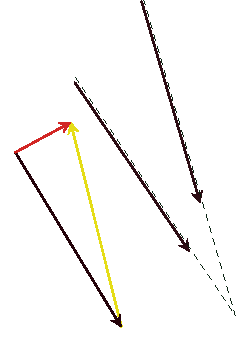
\includegraphics[width=0.8\textwidth]{part1/relativi/FIG/f113.pdf}
\begin{picture}(0,0)(110,0)
\scriptsize{
\put(40,135){${\rm d}\theta$}
\put(3,98){\rotatebox{28}{${\rm d}{\bm v}_{\scriptscriptstyle{{\rm rel}}}$}}
\put(38,65){\rotatebox{-72}{${-{\bm v}_{\scriptscriptstyle{{\rm rel}}}}(t)$}}
\put(0,75){\rotatebox{-58}{${{\bm v}_{\scriptscriptstyle{{\rm rel}}}}(t+{\rm d}t)$}}
\put(70,130){\rotatebox{-72}{${{\bm v}_{\scriptscriptstyle{{\rm rel}}}}(t)$}}
\put(40,115){\rotatebox{-58}{${{\bm v}_{\scriptscriptstyle{{\rm rel}}}}(t+{\rm d}t)$}}
}
\end{picture}
        \caption{\em Cambiamento di direzione della velocit\`a relativa.}
     \label{fig:f113}
\end{minipage}
\end{figure}

\noindent Nella figura \ref{fig:f112} sono rappresentate le due componenti infinitesimali frutto della
differenza tra la velocit\`a di trascinamento al tempo $t+{\rm d}t$ e al tempo $t$.
Non ci occupiamo della componente normale
${\rm d}{{\bm v}_{\scriptscriptstyle{{\rm tr}}}}_{\scriptscriptstyle{n}}$, in quanto a noi gi\`a
nota.
Il lettore pi\`u diligente pu\`o tornare alla figura \ref{fig:f18} e ricavare anche in questo caso
la formula della accelerazione centripeta \ref{e126}.
La velocit\`a infinitesimale 
${{\rm d}{{\bm v}_{\scriptscriptstyle{{\rm tr}}}}}_{\scriptscriptstyle{t}}$ \`e invece
di nostro interesse: tale variazione della velocit\`a tangenziale si esprime come
\begin{equation}
{{\rm d}{{\bm v}_{\scriptscriptstyle{{\rm tr}}}}}_{\scriptscriptstyle{t}}=
\omega[(r -{\rm d}r) - (r)]\hat{{\bm t}}\,,
\label{e139}
\end{equation}
\noindent dove $\hat{\bm t}$ \`e il versore tangente, gi\`a altre volte incontrato (equazione \ref{e119}). Sapendo poi che che la differenza tra i raggi dopo 
un intervallo di tempo ${\rm d}t$ sar\`a ${\rm d} r= |{\bm v}_{\scriptscriptstyle{{\rm rel}}}|
{\rm d}t$, possiamo scrivere 
\begin{equation}
{{\rm d}{{\bm v}_{\scriptscriptstyle{{\rm tr}}}}}_{\scriptscriptstyle{t}}=
-\omega
(|{\bm v}_{\scriptscriptstyle{{\rm rel}}}|{\rm d}t)\,
\hat{{\bm t}}\,,
\label{e140}
\end{equation}
\noindent o anche
\begin{equation}
{{{{\rm d}{{\bm v}_{\scriptscriptstyle{{\rm tr}}}}}_{\scriptscriptstyle{t}}}\over{{\rm d}t}}=
{\bm \omega} \times
{\bm v}_{\scriptscriptstyle{{\rm rel}}}=
{{\bm a}_{\scriptscriptstyle{{\rm cor}}}\over{2}}\,.
\label{e141}
\end{equation}
\noindent Abbiamo cos\`i individuato la natura di met\`a dell'accelerazione
di {\em Coriolis}: essa deriva dalla costrizione subita dal nostro punto osservato a
cambiare raggio sul disco del pavimento, e di conseguenza 
velocit\`a di trascinamento. Questo d\`a conto
di uno dei monomi dell'espressione dell'accelerazione di {\em Coriolis}.
Veniamo ora alla figura \ref{fig:f113} e consideriamo che la velocit\`a relativa, nell'intervallo di
tempo ${\rm d}t$, cambia direzione, ruotando di un angolo pari
a ${\rm d} \theta=\omega{\rm d}t$. 
La variazione della velocit\`a relativa risulta pertanto essere
\begin{equation}
{\rm d}{\bm v}_{\scriptscriptstyle{{\rm rel}}}=
-\omega {\rm d}t 
|{\bm v}_{\scriptscriptstyle{{\rm rel}}}|\hat{\bm t}\,,
\label{e142}
\end{equation}
\noindent quindi 
\begin{equation}
{{\rm d}{\bm v}_{\scriptscriptstyle{{\rm rel}}}\over{\rm d}t}=
{\bm \omega}\times 
{\bm v}_{\scriptscriptstyle{{\rm rel}}}=
{{\bm a}_{\scriptscriptstyle{{\rm cor}}}\over{2}}\,,
\label{e143}
\end{equation}
\noindent che \`e il secondo (o il primo?) monomio dell'accelerazione di {\em Coriolis}.
Cos\`i tale accelerazione, dapprima introdotta
mediante un calcolo formale (derivando la \ref{e130} si \`e ottenuta
la \ref{e134}), si ricava ora mediante le osservazioni test\'e svolte e si
intravede la giustificazione dei suoi due monomi identici: essi sono
da ricondurre a due diverse conseguenze provocate e subite dalla velocit\`a
relativa durante la rotazione del sistema di riferimento relativo.
Possiamo aggiungere che tale chiarimento \`e stato molto
caro all'autore una volta scovato, stampato con tipi minori e con stile
incomparabilmente pi\`u elegante del nostro, su \cite{sesini1}, pag. 11.
Ma anche queste delucidazioni possono lasciare un po' di amaro in bocca per via di ulteriori dubbi che possono sorgere:
cosa succede ai due pluricitati monomi quando la velocit\`a relativa \`e tangente alle circonferenze
del piatto della giostra anzich\'e essere radiale? Che fine fa in tal caso il monomio che
esiste in virt\`u della diminuzione o dell'aumento delle circonferenze percorse nel sistema
relativo? Si riduce forse a zero? Proprio cos\`i! E l'altro monomio, quello dovuto al
cambiamento di direzione della velocit\`a relativa, raddoppia: la dimostrazione di
questa affermazione \`e lasciata come esercizio al lettore.
E cosa succede nelle situazioni intermedie? Cio\`e quando
la velocit\`a relativa non \`e n\'e radiale n\'e tangenziale? Conviene qui
tagliar corto: i procedimenti
matematici servono proprio a questo: la \ref{e134} \`e stata ricavata correttamente
dalla \ref{e130} perci\`o risulta sempre valida. Le altre considerazioni, meno rigorose,
basate su circostanze particolari, servono a stimolare e svegliare l'intuito, ci
fanno conoscere gli attori, solitamente austeri e scontrosi, della matematica con
maggior confidenza.

\section{Ulteriori Precisazioni}

\noindent Ancora qualche parola su questa particolare grandezza cinematica. Anche se
non \`e qui il luogo per trattare argomenti di {\em dinamica}, tutti conosciamo
gli effetti delle accelerazioni sulle masse: esse fanno nascere le {\em forze di inerzia}.
Bench\'e i fisici chiamino queste forze, e non senza ragione,
 ``apparenti'', i loro effetti sono ben noti
ai passeggeri che stanno spesso
in piedi, anzich\'e seduti sugli autobus. Bene, le forze di inerzia legate alle accelerazioni di {\em Coriolis}
provocano particolari azioni dinamiche: sono quelle che al ritrarre o allo stendere
delle braccia del pattinatore ne aumentano o ne diminuiscono
la sua velocit\`a angolare quando piroetta;
esse provocano la circolazione dei venti sul nostro pianeta,
i vortici dei cicloni, e tanti altri effetti analoghi.

\section{Due Esempi Significativi}
\label{par:esempi_moti_rel}

\noindent Abbiamo visto che la soluzione del problema dei
moti relativi si trova in due equazioni che riguardano rispettivamente velocit\`a
e accelerazioni, \ref{e133} e \ref{e138}, ciascuna delle quali mette d'accordo le osservazioni
svolte nei rispettivi sistemi di riferimento, quello assoluto e quello relativo.
Tutte le volte che disponiamo di relazioni di uguaglianza 
siamo autorizzati
a trasformarle in altrettante equazioni
nelle quali qualche termine potr\`a essere incognito.
D'altra parte sappiamo che, dato un sistema di
equazioni tra loro indipendenti, possiamo ricavare il valore delle incognite
se il loro numero uguaglia quello delle relazioni che le legano tra loro.
Desideriamo provare a sfruttare questa attitudine delle uguaglianze \ref{e133} e \ref{e138} per
ricavare alcune grandezze cinematiche incognite
nei due problemi raffigurati nelle figure
\ref{fig:f114} e \ref{fig:f115}.
Andiamo con ordine e cominciamo dalla scala a pioli appoggiata a un muro
che scivola sul pavimento con velocit\`a e accelerazione date,
${{\bm v}_{\scriptscriptstyle{A}}}$ e ${{\bm a}_{\scriptscriptstyle{A}}}$, come rappresentato in figura \ref{fig:f114}.


\begin{figure}[hbt]
\centering
\begin{minipage}[b]{0.48\textwidth}
\centering
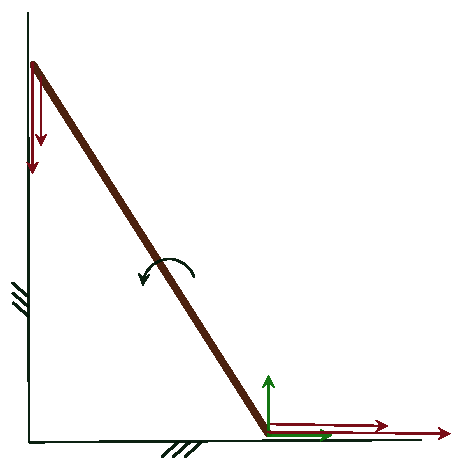
\includegraphics[width=0.8\textwidth]{part1/relativi/FIG/f114.pdf}
\begin{picture}(0,0)(130,0)
\scriptsize{
\put(-9,133){$y$}
\put(-2,123){$B$}
\put(1,92){${{\bm a}_{\scriptscriptstyle{B}}}$}
\put(-18,90){${{\bm v}_{\scriptscriptstyle{B}}}$}
\put(36,66){$\omega$}
\put(91,17){${{\bm v}_{\scriptscriptstyle{A}}}$}
\put(109,15){${{\bm a}_{\scriptscriptstyle{A}}}$}
\put(62,1){$A$}
\put(-9,1){$O$}
\put(68,28){$y'$}
\put(81.5,3){$x'$}
\put(105,3){$x$}
}
\end{picture}
\caption{\em Slittamento di una scala appoggiata a un muro.}
 \label{fig:f114}
\end{minipage}\hfill
\begin{minipage}[b]{0.48\textwidth}
\centering
      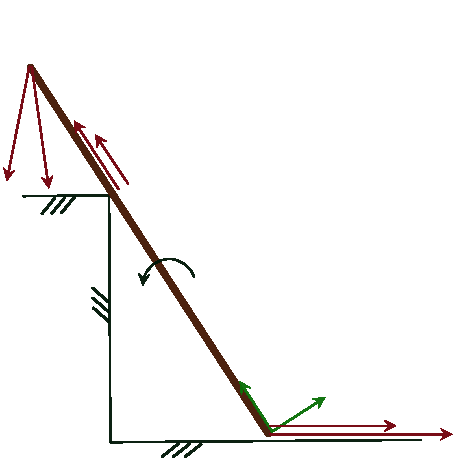
\includegraphics[width=0.8\textwidth]{part1/relativi/FIG/f115.pdf}
\begin{picture}(0,0)(129,0)
\scriptsize{
\put(-2,123){$B$}
\put(2,87){${{\bm a}_{\scriptscriptstyle{B}}}$}
\put(-25,90){${{\bm v}_{\scriptscriptstyle{B}}}$}
\put(24,88){${{\bm v}_{\scriptscriptstyle{P}}}_{\scriptscriptstyle{{\rm rel}}}$}
\put(10,105){${{\bm a}_{\scriptscriptstyle{P}}}_{\scriptscriptstyle{{\rm rel}}}$}
\put(11,74){$P$}
\put(36,66){$\omega$}
\put(11,40){$y$}
\put(92,17){${{\bm v}_{\scriptscriptstyle{A}}}$}
\put(109,15){${{\bm a}_{\scriptscriptstyle{A}}}$}
\put(11,1){$O$}
\put(62,1){$A$}
\put(60,28){$y'$}
\put(83,22){$x'$}
\put(105,3){$x$}
}
\end{picture}
        \caption{\em Slittamento di una scala sopra la sommit\`a di un muro.}
     \label{fig:f115}
\end{minipage}
\end{figure}

\noindent Ci poniamo il problema di trovare velocit\`a e accelerazione del punto $B$, cio\`e
${{\bm v}_{\scriptscriptstyle{B}}}$ e 
${{\bm a}_{\scriptscriptstyle{B}}}$, conoscendo 
${{\bm v}_{\scriptscriptstyle{A}}}$ e 
${{\bm a}_{\scriptscriptstyle{A}}}$, ossia le grandezze cinematiche del
punto $A$.
Esprimiamo le grandezze cinematiche assolute di $B$ tramite le grandezze
 relative 
appartenenti al sistema di riferimento $(x',y')$. Assumiamo in questo caso
(ma su questa scelta torneremo) che il sistema relativo trasli e si mantenga centrato in $A$.
Nel sistema relativo $(x',y')$ si osserva $B$ 
percorrere degli archi di circonferenza con centro $A$. Riprendendo la \ref{e133} possiamo scrivere
\begin{equation}
{\bm v}_{\scriptscriptstyle{{\rm ass}}}=
{\bm v}_{\scriptscriptstyle{{\rm rel}}}+
{\bm v}_{\scriptscriptstyle{{\rm tr}}}\,,
\label{e144}
\end{equation}
\noindent cio\`e
\begin{equation}
{{\bm v}_{\scriptscriptstyle{B}}}= 
{{\bm v}_{\scriptscriptstyle{B}}}_{\scriptscriptstyle{{\rm rel}}}+ 
{{\bm v}_{\scriptscriptstyle{A}}}\,. 
\label{e145}
\end{equation}
\noindent L'equazione \ref{e145} contiene due incognite, i vettori
${{\bm v}_{\scriptscriptstyle{B}}}$ e 
${{\bm v}_{\scriptscriptstyle{B}}}_{\scriptscriptstyle{{\rm rel}}}$. 
Ma tali grandezze non sono
completamente sconosciute in quanto la loro direzione \`e nota. Siamo pertanto di fronte
a un'equazione vettoriale (che nel piano vale due equazioni scalari) che contiene due incognite, i moduli dei vettori che non conosciamo.
Stabilito quindi che il numero delle incognite non eccede il numero delle equazioni, potremmo
lasciare al lettore il compito di individuare 
uno dei vari metodi per risolvere la \ref{e145}.
Preferiamo per\`o dare un cenno del metodo grafico che si potrebbe seguire,
metodo forse non molto efficiente ma a nostro parere molto istruttivo.
\begin{wrapfigure}{r}{0.35\textwidth}
      \begin{center}
      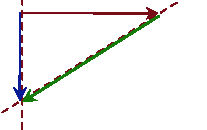
\includegraphics[width=0.30\textwidth]{part1/relativi/FIG/f116.pdf}
     \end{center}
\begin{picture}(0,0)(0,0)
\scriptsize{
\put(40,91){${{\bm v}_{\scriptscriptstyle{A}}}$}
\put(6,55){${{\bm v}_{\scriptscriptstyle{B}}}$}
\put(36,44){${{\bm v}_{\scriptscriptstyle{B}}\scriptscriptstyle{{\rm rel}}}$}
\put(61,59){\rotatebox{30}{${\scriptstyle{{\rm dir}}}{\scriptscriptstyle{\perp AB}}$}}
\put(13,30){\rotatebox{-90}{${\scriptstyle{{\rm dir}}}{\scriptscriptstyle{\parallel OB}}$}}
}
\end{picture}
        \caption{\em Soluzione grafica di un'equazione vettoriale.}
     \label{fig:f116}
\end{wrapfigure}
\noindent Con riferimento alla figura \ref{fig:f116} tracciamo dapprima il vettore noto 
${{\bm v}_{\scriptscriptstyle{A}}}$. Si tracciano quindi per i suoi estremi
le due direzioni cospicue indicate nella stessa figura.
Non ha alcuna importanza se la direzione parallela a $OB$ viene riportata sulla
coda del vettore noto oppure sulla sua testa e naturalmente lo stesso vale per l'altra direzione nota.
La soluzione consta nell'ammettere
che l'unica configurazione in cui i vettori incogniti
giacciano sulle direzioni tracciate e soddisfino
la relazione \ref{e145} risulta essere quella
riportata in figura, e la chiusura del triangolo
costituisce la soluzione dell'equazione vettoriale.
Una volta determinate
le velocit\`a incognite
si pu\`o senza fatica ricavare
il modulo della velocit\`a angolare della scala
 dalla relazione
$|{{\bm v}_{\scriptscriptstyle{B}}\scriptscriptstyle{{\rm rel}}}|=\omega\overrightarrow{|{AB}|}$;
tenendo quindi presente che la sua direzione non pu\`o 
che essere ortogonale al piano del moto, il suo
verso dovr\`a soddisfare la relazione
${{\bm v}_{\scriptscriptstyle{B}}\scriptscriptstyle{{\rm rel}}}=\bm{\omega}\times\overrightarrow{AB}$. 


\noindent Passiamo alle accelerazioni. In virt\`u del fatto che il sistema di riferimento relativo trasla, scrivendo la \ref{e138} il termine dell'accelerazione di {\em Coriolis} sar\`a assente. 
Avremo pertanto


\begin{equation}
{{\bm a}_{\scriptscriptstyle{B}}}= 
{{\bm a}_{\scriptscriptstyle{B}}}_{\scriptscriptstyle{{\rm rel}}}+
{{\bm a}_{\scriptscriptstyle{A}}}\,.
\label{e146}
\end{equation}

\noindent Conviene per\`o scrivere il termine
${{\bm a}_{\scriptscriptstyle{B}}}_{\scriptscriptstyle{{\rm rel}}}$ come somma delle sue due
componenti: quella avente direzione parallela alla scala e diretta verso $A$ (componente normale) e quella ortogonale alla scala stessa

\begin{equation}
{{\bm a}_{\scriptscriptstyle{B}}}= 
-\omega^2 \overrightarrow{AB} + \dot{\omega}|\overrightarrow{AB}|\widehat{{\perp{AB}}}+
{{\bm a}_{\scriptscriptstyle{A}}}\,,
\label{e147}
\end{equation}

\noindent dove il versore
$\widehat{{\perp{AB}}}$ sta ad indicare che la direzione del penultimo termine, al contrario del suo
modulo, \`e nota e proviene dal prodotto vettoriale
${{{\bm a}_{\scriptscriptstyle{B}}}_{\scriptscriptstyle{{\rm rel}}}}_{\scriptscriptstyle{(t)}}=
\dot{\bm\omega}\times\overrightarrow{AB}$,
pertanto essa risulta perpendicolare alla nostra scala.
Anche la direzione del vettore incognito ${{\bm a}_{\scriptscriptstyle{B}}}$
\`e nota ed \`e l'unica che il moto di strisciamento sul
muro verticale gli consenta.
Gli altri due termini, ${{\bm a}_{\scriptscriptstyle{A}}}$ e
${{{\bm a}_{\scriptscriptstyle{B}}}_{\scriptscriptstyle{{\rm rel}}}}_{\scriptscriptstyle{(n)}}=-\omega^2 \overrightarrow{AB}$, sono
invece completamente noti.
Ricadiamo cos\`i ancora nel caso di un'equazione vettoriale dove le incognite sono i moduli di due vettori; in questo frangente,
numerando i termini senza badare al segno di uguaglianza, risultano essere il primo e il terzo.
Una possibile soluzione \`e quindi di nuovo
lo schema grafico di figura \ref{fig:f116}, magari con l'avvertenza di produrre in
anticipo la somma dei due vettori noti. 
Occorre solo accennare che una volta ricavato
il terzo termine, 
${{{\bm a}_{\scriptscriptstyle{B}}}_{\scriptscriptstyle{{\rm rel}}}}_{\scriptscriptstyle{(t)}}=
\dot{\omega}|\overrightarrow{AB}|\widehat{{\perp{AB}}}$, risulter\`a noto anche
il modulo  dell'accelerazione 
angolare della scala $\dot{\omega}$; la sua direzione sar\`a ortogonale
al piano del moto e il suo verso dovr\`a
essere tale da produrre il
valore corretto di 
${{{\bm a}_{\scriptscriptstyle{B}}}_{\scriptscriptstyle{{\rm rel}}}}_{\scriptscriptstyle{(t)}}$
tramite il prodotto vettoriale con $\overrightarrow{AB}$.


\noindent Esaminiamo ora la scala della figura \ref{fig:f115} che, anzich\'e appoggiarsi al muro verticale
mediante il suo estremo $B$, appoggia in un suo punto imprecisato sulla sommit\`a del muro nel
punto (del muro) $P$. Abbiamo scelto di relazionarci con un osservatore relativo
che, oltre a traslare con il punto $A$, ruota mantenendo uno dei suoi assi diretto
lungo la scala.
Anche qui, le incognite sono velocit\`a e accelerazione del punto $B$, note la velocit\`a
e l'accelerazione del punto $A$\footnote
{
Il lettore, qualora fosse interessato, pu\`o provare
a scambiare le grandezze incognite con quelle note e viceversa, per rendersi
conto che, non solo la soluzione non cambia a livello concettuale, ma persino
nelle equazioni e nei disegni le grandezze coinvolte
rimarranno invariate nella sostanza.
}.
Ancora una volta partiamo dalle velocit\`a ma, anzich\'e tentare di coinvolgere subito
la grandezza incognita  
${{\bm v}_{\scriptscriptstyle{B}}}$,
proviamo a calcolare la velocit\`a del punto $P$, che deve essere nulla essendo
$P$ un punto appartenente al muro.
In tal caso, la \ref{e133} diventa

\begin{equation}
{{\bm v}_{\scriptscriptstyle{P}}}=0= 
{{\bm v}_{\scriptscriptstyle{P}}}_{\scriptscriptstyle{{\rm rel}}}+ 
{{\bm v}_{\scriptscriptstyle{A}}}+
{\omega}|\overrightarrow{AP}|\widehat{{\perp{AP}}}\,,
\label{e148}
\end{equation}

\noindent dove 
${{\bm v}_{\scriptscriptstyle{P}}}_{\scriptscriptstyle{{\rm rel}}}$ ha modulo incognito e direzione lungo la scala,
${{\bm v}_{\scriptscriptstyle{A}}}$ \`e un vettore noto e l'altra componente di trascinamento
${{\bm v}_{\scriptscriptstyle{{\rm tr}}}}_{\scriptscriptstyle{{\rm (n)}}}=
{\omega}|\overrightarrow{AP}|\widehat{{\perp{AP}}}$
ha modulo incognito e direzione ortogonale la scala.
Di nuovo una equazione vettoriale dove le direzioni sono tutte note mentre sono incogniti due dei tre moduli. Si possono quindi ricavare sia la velocit\`a relativa di $P$,
${{\bm v}_{\scriptscriptstyle{P}}}_{\scriptscriptstyle{{\rm rel}}}$, sia il
modulo della velocit\`a angolare
$\omega$; il vettore $\bm \omega$ sar\`a come al solito ortogonale
al piano del moto e il suo verso dovr\`a soddisfare la relazione vettoriale
${{\bm v}_{\scriptscriptstyle{{\rm tr}}}}_{\scriptscriptstyle{{\rm (n)}}}=
{\bm\omega}\times\overrightarrow{AP}$.
La velocit\`a del punto
$B$ sar\`a 
\begin{equation}
{{\bm v}_{\scriptscriptstyle{B}}}= 
{{\bm v}_{\scriptscriptstyle{A}}}+
\bm\omega\times\overrightarrow{AB}\,.
\label{e149}
\end{equation}

\noindent Passando alle accelerazioni dovremo in questo caso fare i conti anche con l'accelerazione di {\em Coriolis}, in quanto il sistema relativo ruota con
velocit\`a angolare $\bm\omega$, ormai nota. Al fine di riportare
le espressioni delle accelerazioni ci avvarremo, anche in questo caso,
delle loro componenti, quando queste saranno pi\`u semplici da calcolare.
Dunque, con riferimento alla \ref{e139},
avremo per l'accelerazione del punto $P$
\begin{equation}
{{\bm a}_{\scriptscriptstyle{P}}}=0= 
{{\bm a}_{\scriptscriptstyle{P}}}_{\scriptscriptstyle{{\rm rel}}}+ 
{{\bm a}_{\scriptscriptstyle{A}}}
-\omega^2 \overrightarrow{AP} + \dot{\omega}|\overrightarrow{AP}|\widehat{{\perp{AP}}}+
2{\bm \omega}\times
{{\bm v}_{\scriptscriptstyle{P}}}_{\scriptscriptstyle{{\rm rel}}}\,,
\label{e150}
\end{equation}

\noindent dove il prodotto vettoriale del
termine di {\em Coriolis} ha il solo scopo di indicarne la direzione e il verso. 
Quando la rotazione $\omega$ segue 
le dita della mano destra, il pollice d\`a la direzione e il verso
di $\bm \omega$. Diamo  ora all'indice direzione e verso della velocit\`a
relativa: tenendo le tre dita reciprocamente ortogonali tra
loro, il dito medio fornir\`a la direzione e il verso
dell'accelerazione di {\em Coriolis}. Il procedimento ora indicato
si chiama {\em regola della mano destra}\index{regola della mano destra}
per il prodotto vettoriale.
Dei cinque termini della \ref{e150} tre sono completamente noti
\begin{equation}
{\rm termine\, noto}\equiv
{{\bm a}_{\scriptscriptstyle{A}}}
-\omega^2 \overrightarrow{AP} + 
2{\bm \omega}\times
{{\bm v}_{\scriptscriptstyle{P}}}_{\scriptscriptstyle{{\rm rel}}}\,,
\label{e151}
\end{equation}

\noindent mentre l'accelerazione relativa di $P$ e la componente tangenziale dell'accelerazione di trascinamento presentano modulo incognito
e direzione nota.
Ancora una volta, il riferimento per la soluzione
pu\`o essere lo schema di figura \ref{fig:f116},
che permette di ricavare i moduli delle
due accelerazioni incognite e di conseguenza ci consentir\`a di conoscere
il modulo dell'accelerazione angolare della scala $\dot{\omega}$ prima e poi
$\dot{\bm\omega}$.
Infine si pu\`o ottenere l'accelerazione dell'estremo 
$B$ della scala dalla seguente
\begin{equation}
{{\bm a}_{\scriptscriptstyle{B}}}= 
{{\bm a}_{\scriptscriptstyle{A}}}
-\omega^2 \overrightarrow{AB} + \dot{\bm\omega}\times\overrightarrow{AB}\,.
\label{e152}
\end{equation}


\noindent A conclusione di questo breve esempio di applicazione del teorema di {\em Coriolis} sorge spontanea
una domanda: gli esercizi di figura \ref{fig:f114} e di figura \ref{fig:f115}
appaiono molto simili; come abbiamo dunque fatto ad affibbiare un sistema
relativo traslante al primo, mentre nel secondo caso scegliamo un sistema
relativo traslante-rotante?
La decisione da prendere in tal senso sta forse alla nostra discrezione?
Purtroppo no. Se utilizzassimo
un sistema relativo rotante anche nel primo caso, ci accorgeremmo subito
che la sua rotazione non sarebbe di utilit\`a alcuna. 
Nel secondo caso, introducendo un riferimento relativo che trasla senza ruotare,
non sarebbe possibile giungere alla soluzione.
Una linea guida per scegliere tra il sistema relativo semplicemente traslante e quello
che ruota ``incollato'' a qualche corpo rigido pu\`o essere la 
seguente: tutte le volte che le grandezze relative non possono
in alcun modo essere rappresentate come prodotte dal trascinamento (un classico esempio
\`e la velocit\`a radiale della formica sul piatto della giostra)  \`e 
indispensabile l'introduzione di un sistema di riferimento relativo che, oltre eventualmente a traslare, ruoti.

\section{Ulteriori Considerazioni sui Moti Relativi}

Nelle applicazioni pratiche \`e uso comune riferire i moti a sistemi che si
qualificano come assoluti quando sono in qualche modo fissati a qualche
cosa di molto grande, in generale il nostro pianeta, mentre 
si qualificano come relativi sistemi di riferimento che sono in moto
rispetto alla Terra. Al fine di contrastare (in modo pacifico) tale punto 
di vista,
oltre a tirare in ballo il valido argomento, che quasi tutti conoscono,
che la Terra si muove, ci preme sottolineare che gli unici
moti sperimentalmente rintracciabili sono quelli relativi.
Un insieme di corpi rigidi \`e un teatro nel quale (quando i vincoli
lo permettono) i vari attori posseggono campi di velocit\`a misurabili soltanto
rispetto agli altri corpi.

\begin{figure}[ht]
	\begin{center}
      		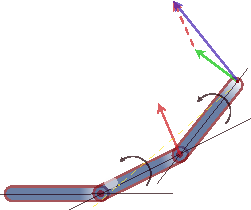
\includegraphics[width=0.9\textwidth]{part1/relativi/FIG/arnold_kennedy.pdf}
	\end{center}
\begin{picture}(0,0)(-55,-50)
\scriptsize{
	\put(0,14){corpo $1$}
	\put(234,72){\rotatebox{53}{corpo $3$}}
	\put(108,22){\rotatebox{24}{corpo $2$}}
	\put(115,48){$\omega_{21}$}
	\put(87,14){$A$}
	\put(198,28){$B$}
	\put(261,138){$P$}
	\put(107,7){$C$}
	\put(230,129){$\omega_{32}$}
	\put(222,166){\rotatebox{-38}{${\bm\omega}_{32}\times\overrightarrow{BP}$}}
	\put(235,189){${{\bm v}_{\scriptscriptstyle{P}}}_{\scriptscriptstyle 1}$}
	\put(162,117){${v_{\scriptscriptstyle B}}_{\scriptscriptstyle 1}$}
}
\end{picture}
	\caption{\em Allineamento dei tre centri di rotazione.}
     \label{fig:arnold_kennedy}
\end{figure}

\noindent Cosicch\'e, considerando la figura \ref{fig:arnold_kennedy}, 
possiamo riferire il moto di ciascuno dei tre corpi a ciascuno dei due
rimanenti. In figura si nota che il corpo $1)$ e il corpo $2)$ sono
tra loro uniti da un giunto rotoidale e cos\`i accade per il corpo $2)$ e
il corpo $3)$. Sappiamo quindi che il moto di $2)$ relativamente a $1)$
sar\`a rotatorio con centro $A$ (e naturalmente lo stesso vale per il 
moto di $1)$ rispetto a $2)$), cos\`i come il moto di $3)$ attorno
a $2)$ sar\`a anch'esso rotatorio con centro $B$. 
Volendo descrivere il moto di $3)$ rispetto a $1)$ richiamiamo la regola della
composizione delle velocit\`a (\ref{e133}):
\begin{equation}
{\bm v}_{\rm ass} = {\bm v}_{\rm tr} + {\bm v}_{\rm rel}\,.
\nonumber
\end{equation}

\noindent Pensando come assoluta la velocit\`a
di $P$, punto  appartenente al corpo  $3)$,
relativa al corpo $1)$, ${{\bm v}_{\scriptscriptstyle P}}_{\scriptscriptstyle 1}$, con ovvio significato dei 
simboli avremo  
\begin{equation}
{{\bm v}_{\scriptscriptstyle P}}_{\scriptscriptstyle 1} = {{\bm v}_{\scriptscriptstyle B}}_{\scriptscriptstyle 1} + {{\bm v}_{\scriptscriptstyle P}}_{\scriptscriptstyle 2}\,.
\label{eq:vel_p}
\end{equation}

\noindent La \ref{eq:vel_p} ci dice che la stessa 
${{\bm v}_B}_1$, componente di trascinamento, \`e anche la velocit\`a del
particolare punto del corpo $3)$ coincidente con $B$.
Questa informazione, da sola, ci d\`a la certezza che il centro di istantanea
rotazione del corpo $3)$ nel moto relativo a $1)$, dovendo stare
sulla normale a tale vettore,
giacer\`a da
qualche parte sulla retta che passa per i punti $A$ e $B$.
Se desideriamo individuare il centro di istantanea rotazione $C$ del
corpo $3)$ rispetto al corpo $1)$ (e viceversa),
sempre tramite la \ref{eq:vel_p} calcoliamo la velocit\`a
del generico punto $P$ del corpo $3)$ rispetto al corpo $1)$.
Una volta identificato il vettore
${{\bm v}_{\scriptscriptstyle P}}_{\scriptscriptstyle 1}$, 
come in figura, baster\`a condurre la perpendicolare al suo piede e
$C$ risulter\`a determinato dall'intersezione con
la retta che passa per i punti $A$ e $B$.
Il punto $C$ \`e il centro di rotazione istantaneo
del moto relativo tra $1)$ e $3)$\footnote{Risulta essere 
{\em istantaneo} in quanto non abbiamo premesso alcuna ipotesi circa la
costanza o meno della velocit\`a angolare 
$\omega_{32}$, per questo la posizione di $C$
relativa ai tre corpi pu\`o variare nel tempo. Se tale velocit\`a angolare fosse costante,
il centro $C$ non si sposterebbe.}.
In questa analisi,
l'esistenza dei vincoli rotoidali $A$ e $B$
\`e stata sfruttata solamente per scrivere 
la \ref{eq:vel_p}, la quale sarebbe corretta anche se $A$
fosse il centro istantaneo di rotazione di $2)$ 
rispetto a $1)$ e $B$ il centro istantaneo del moto relativo tra $2)$ e $3)$.
Questo notevole risultato, che vede i tre centri istantanei dei moti relativi di
tre corpi sempre allineati tra loro, costituisce il {\em teorema di
Aronhold-Kennedy}\index{teorema!di Kennedy}. 
La tesi di questo teorema viene spesso utilizzata nell'analisi cinematica
che gli ingegneri civili eseguono sulle strutture:
se tre corpi, tra loro connessi,
 presentano centri istantanei di rotazione relativi allineati,
tali corpi hanno una possibilit\`a (almeno in quell'istante) di muoversi
l'uno rispetto all'altro, situazione questa quasi sempre da evitarsi
nelle costruzioni.
\newpage
\thispagestyle{empty}
\null

\endinput
